\title{RAM}
\begin{document}

\section{Types of RAM}

\begin{frame}{Types of RAM}
  We will explore the two main types of RAM.
  \begin{itemize}
    \item Both types of RAM are arrays of bits, like ROM.
    \item Both can be specified with n address inputs and b data inputs/outputs, storing $2^n$xb bits.
  \end{itemize}
  \begin{block}{Static RAM (SRAM)}
    Once data is written to SRAM, it can be read at any time, as long is power is continuously applied to the SRAM.
  \end{block}
  \begin{block}{Dynamic RAM (DRAM)}
    The data stored in DRAM must be periodically refreshed (read and written again) or it will be lost.
  \end{block}
\end{frame}

\section{Static RAM}

\subsection{Static RAM Behavior}

\begin{frame}{Static RAM (SRAM)}
  The interface to SRAM is very similar to ROM, with the addition of a few signals.\\
  \begin{center}
    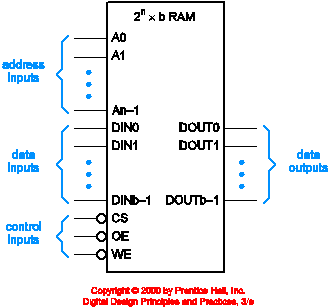
\includegraphics[scale=0.4]{SRAMSchematic}
  \end{center}
\end{frame}

\begin{frame}{Modes of operation}
  SRAM usually has two modes of operation.
  \begin{columns}
    \begin{column}{6cm}
      \begin{itemize}
        \item [Read] CS and OE are asserted, and the data corresponding to the given address is available on DOUT.
        \item [Write] CS and WE are asserted, and the data on DIN is stored in the location specified by the address given.
      \end{itemize}
    \end{column}
    \begin{column}{5cm}
      \begin{center}
        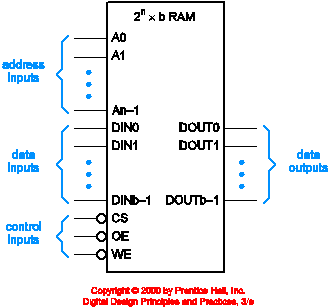
\includegraphics[scale=0.3]{SRAMSchematic}
      \end{center}
    \end{column}
  \end{columns}
\end{frame}

\subsection{Static RAM Structure}

\begin{frame}{Internal implementation}
  Each bit in an SRAM can be implemented using a D latch.\\
  \begin{center}
    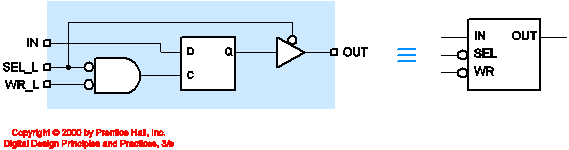
\includegraphics[scale=0.4]{SRAMLogic}
  \end{center}
\end{frame}

\begin{frame}{Array structure}
  \begin{center}
    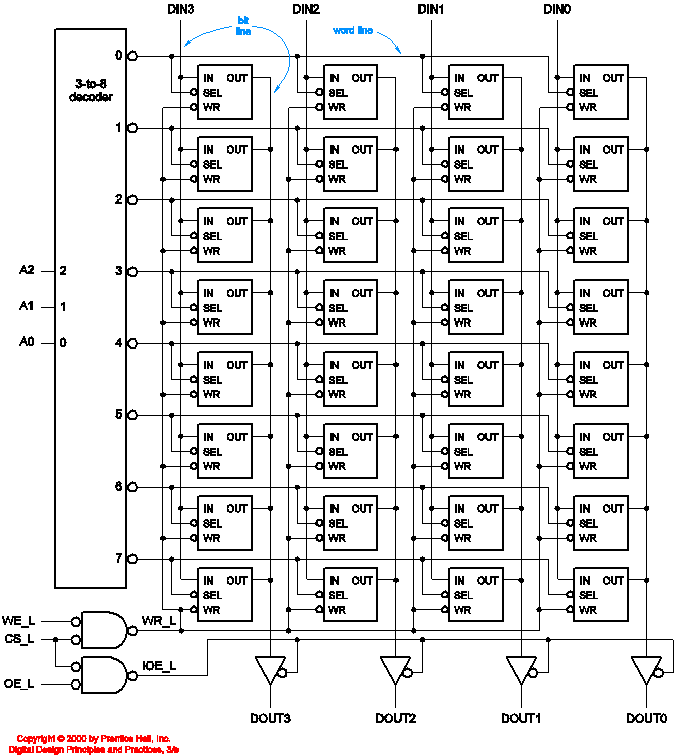
\includegraphics[scale=0.5]{SRAMStructure}
  \end{center}
\end{frame}

\subsection{Static RAM Timing Issues}

\begin{frame}{Timing constraints}
  Since SRAM uses latches internally, we have to adhere to special timing constraints.
  \begin{itemize}
    \item The input data on DIN must be stable for a given length of time before a write cycle is complete.
    \item The address inputs must be set up before and held for a given time after the write cycle occurs to prevent the decoder switching from writing to the wrong location in memory.
    \item A read operation is a combinational function, and is therefore subject to propagation delay.
  \end{itemize}
  Why not use a clock to eliminate these issues?
\end{frame}

\section{Dynamic RAM}

\subsection{Dynamic RAM Structure}

\begin{frame}{Who needs logic gates?}
  Instead of using latches or flip-flops, DRAM stores each bit using one transistor and one capacitor.\\
  \begin{columns}
    \begin{column}{5cm}
      \begin{itemize}
        \item [Write 0] word line high, bit line low
        \item [Write 1] word line high, bit line high
        \item [Read] word line high, bit line halfway
      \end{itemize}
    \end{column}
    \begin{column}{5cm}
      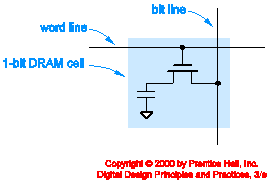
\includegraphics[scale=0.4]{DRAMLogic}
    \end{column}
  \end{columns}
\end{frame}

\begin{frame}{DRAM array layout}
  \begin{center}
    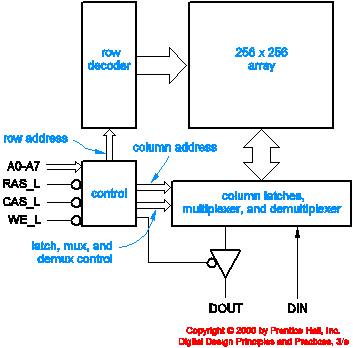
\includegraphics[scale=0.6]{DRAMStructure}
  \end{center}
\end{frame}


\subsection{Dynamic RAM Timing}

\begin{frame}{Refresh scheme}
  After each read operation, the data read is destroyed.  Data is also lost after a given time (about 100 ms).
  \begin{itemize}
    \item After each read, the data read is written again to each bit.
    \item Each bit is periodically refreshed (the data is read and immediately written again).
  \end{itemize}
  \begin{center}
    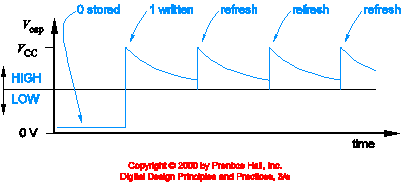
\includegraphics[scale=0.3]{DRAMRefresh}
  \end{center}
  With DRAM, we read and write a large number of bits at a time, to amortize the refresh operations.
\end{frame}

\subsection{Dynamic RAM Timing}

\begin{frame}{DRAM timing}
  \begin{enumerate}
    \item Pre-charge the bit lines to a halfway voltage.
    \item Wait for the pre-charge to complete.
    \item High order address bits are stored in an internal register that selects a row and stores its bits in a row latch.
    \item Wait for the latch to store the data.
    \item The low order address bits select which columns of the row to output.
    \item Wait for the data to be applied to the outputs.
  \end{enumerate}
  During the last step, the RAM is internally writing the data from the row latch back into the memory.
\end{frame}

\begin{frame}{Making RAM faster}
  \begin{block}{Really fast RAM}
    Most PCs use \alert{double data rate} (DDR) SDRAM.  The RAM is faster than normal SDRAM.
  \end{block}
  \begin{itemize}
    \item Data is transfered on both the rising and the falling edges of the clock.
    \item Internally, this requires some exciting clock logic.
  \end{itemize}
  Most DRAM is made up of multiple banks of RAM, that can be accessed in parallel by the memory controller.
\end{frame}

\end{document}
